\documentclass[\report.tex]{subfiles}

\begin{document}
\section{Image Analysis}
\noindent A key requirement for this project was to build a python script allowing JPG images to be read as an array, manipulated and then processed with Python packages such as Sci-Kit Image (skimage) \cite{scikitimage}. Several microstructure images have been used in this project, from a variety of sources including previous research data, scientific literature and the provided database, all with full and sufficient permissions. Images were then pre-processed accordingly through various techniques such as segmentation, removal of noise and measurement testing, before being imported into FE simulations to create a mesh. This section will further detail how this process was undertaken and broken down through the use of test cases to ensure that the python script and skimage were performing accurately and as desired.\\

\noindent The first test case that was carried out was processing an image of a ferritic microstructure taken from the Materials Science and Engineering: An Introduction by W. D. Callister, as seen in Figure \ref{fig:Testcase1} \cite{CallisterJrWilliamD2000MSaE}.
Firstly, an understanding of how to navigate and operate the skimage package was developed, as the software was new to the authors, through testing different algorithms and operations independently on the test image. This included manipulating image colour and contrast, converting the image to grayscale and cropping the image to remove the scale bar. Other features that were tested at this stage was the use of filters such as the Sobel filter, which is commonly used in image processing to emphasise the edges in an image, aiding edge detection algorithms.
A watershed transform was another image processing technique that was trialled at this stage, where the image is treated as a topographical map, with brightness determining elevation of each point and then identifying the lines which run across the peaks to segment the map. Finally, these operations were combined to process the image shown in Figure \ref{fig:Testcase1_2} as effectively as possible, before the measuring tools were used to estimate average grain size.\\


\begin{figure}[!htb]
  \centering
  \begin{minipage}[!htb]{.5\textwidth}
    \centering\captionsetup{width=.8\linewidth}%
    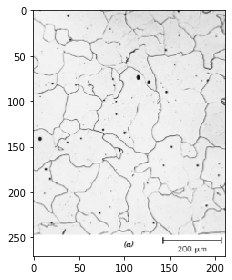
\includegraphics[width=0.6\linewidth, height=0.3\textheight]{Testcase1_initial}
    \caption{A figure showing the initial microstructure image taken from \cite{CallisterJrWilliamD2000MSaE}.}\label{fig:Testcase1}
  \end{minipage}%
  \begin{minipage}[!htb]{.5\textwidth}
    \centering\captionsetup{width=.8\linewidth}%
    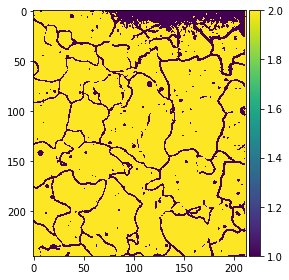
\includegraphics[width=0.65\linewidth, height=0.3\textheight]{testcase1}
    \caption{A figure showing the final image after segmentation and processing.}
    \label{fig:Testcase1_2}
  \end{minipage}
%\caption{}\label{fig:1}
\end{figure}

\pagebreak
\noindent Secondly, in test case 2, the effectiveness of the code developed in the first test case was applied to an image of a thermally etched steel microstructure in Figure \ref{fig:SA508} showing prior austenite grains. This image was taken from previous research by Joshua Collins and authorised by their academic supervisor, Dr Ed Pickering. This microstructure image, as seen below, had previously been the subject of average grain size analysis via the linear intercept method. The average grain size was calculated using the developed image processing Python script and compared with experimental results to assess the accuracy of the approach. The image was processed using many of the techniques tested out previously, with the image first being read before being cropped to remove unfocused areas of the micrograph. The image was then segmented via the application of the Sobel filter, application of markers and then a watershed transform to fill in regions of the elevation map before the grains could finally be segmented and labelled individually. Finally, the image was converted back to gray scale, to allow each grain to be assigned a phase number associated with material properties. This allowed the "image" data to be exported as a numpy array and saved as a Comma Seperated Value (CSV) file for easy importation into the Gmsh meshing software later.\\

\noindent As mentioned previously the successfulness of the second test case was validated by comparing the calculated average grain size from the python algorithm to the previously measured value using the linear intercept method. To do this, the area of each segmented grain in Figure \ref{fig:SA508_2} was measured and then the average diameter of each grain was estimated. This was done by assuming that the grains were perfect circles. Although this is a large assumption which is clearly not true, it yielded excellent results as an average grain size of 23.5 microns was estimated, with the previously measured average of 24.9 microns. Such a small difference in average grain size clearly demonstrates the viability of this approach and provided reassurance that the algorithm could accurately be applied to other images. \\



\begin{figure}[!htb]
  \centering
  \begin{minipage}[!htb]{.5\textwidth}
    \centering\captionsetup{width=.8\linewidth}%
    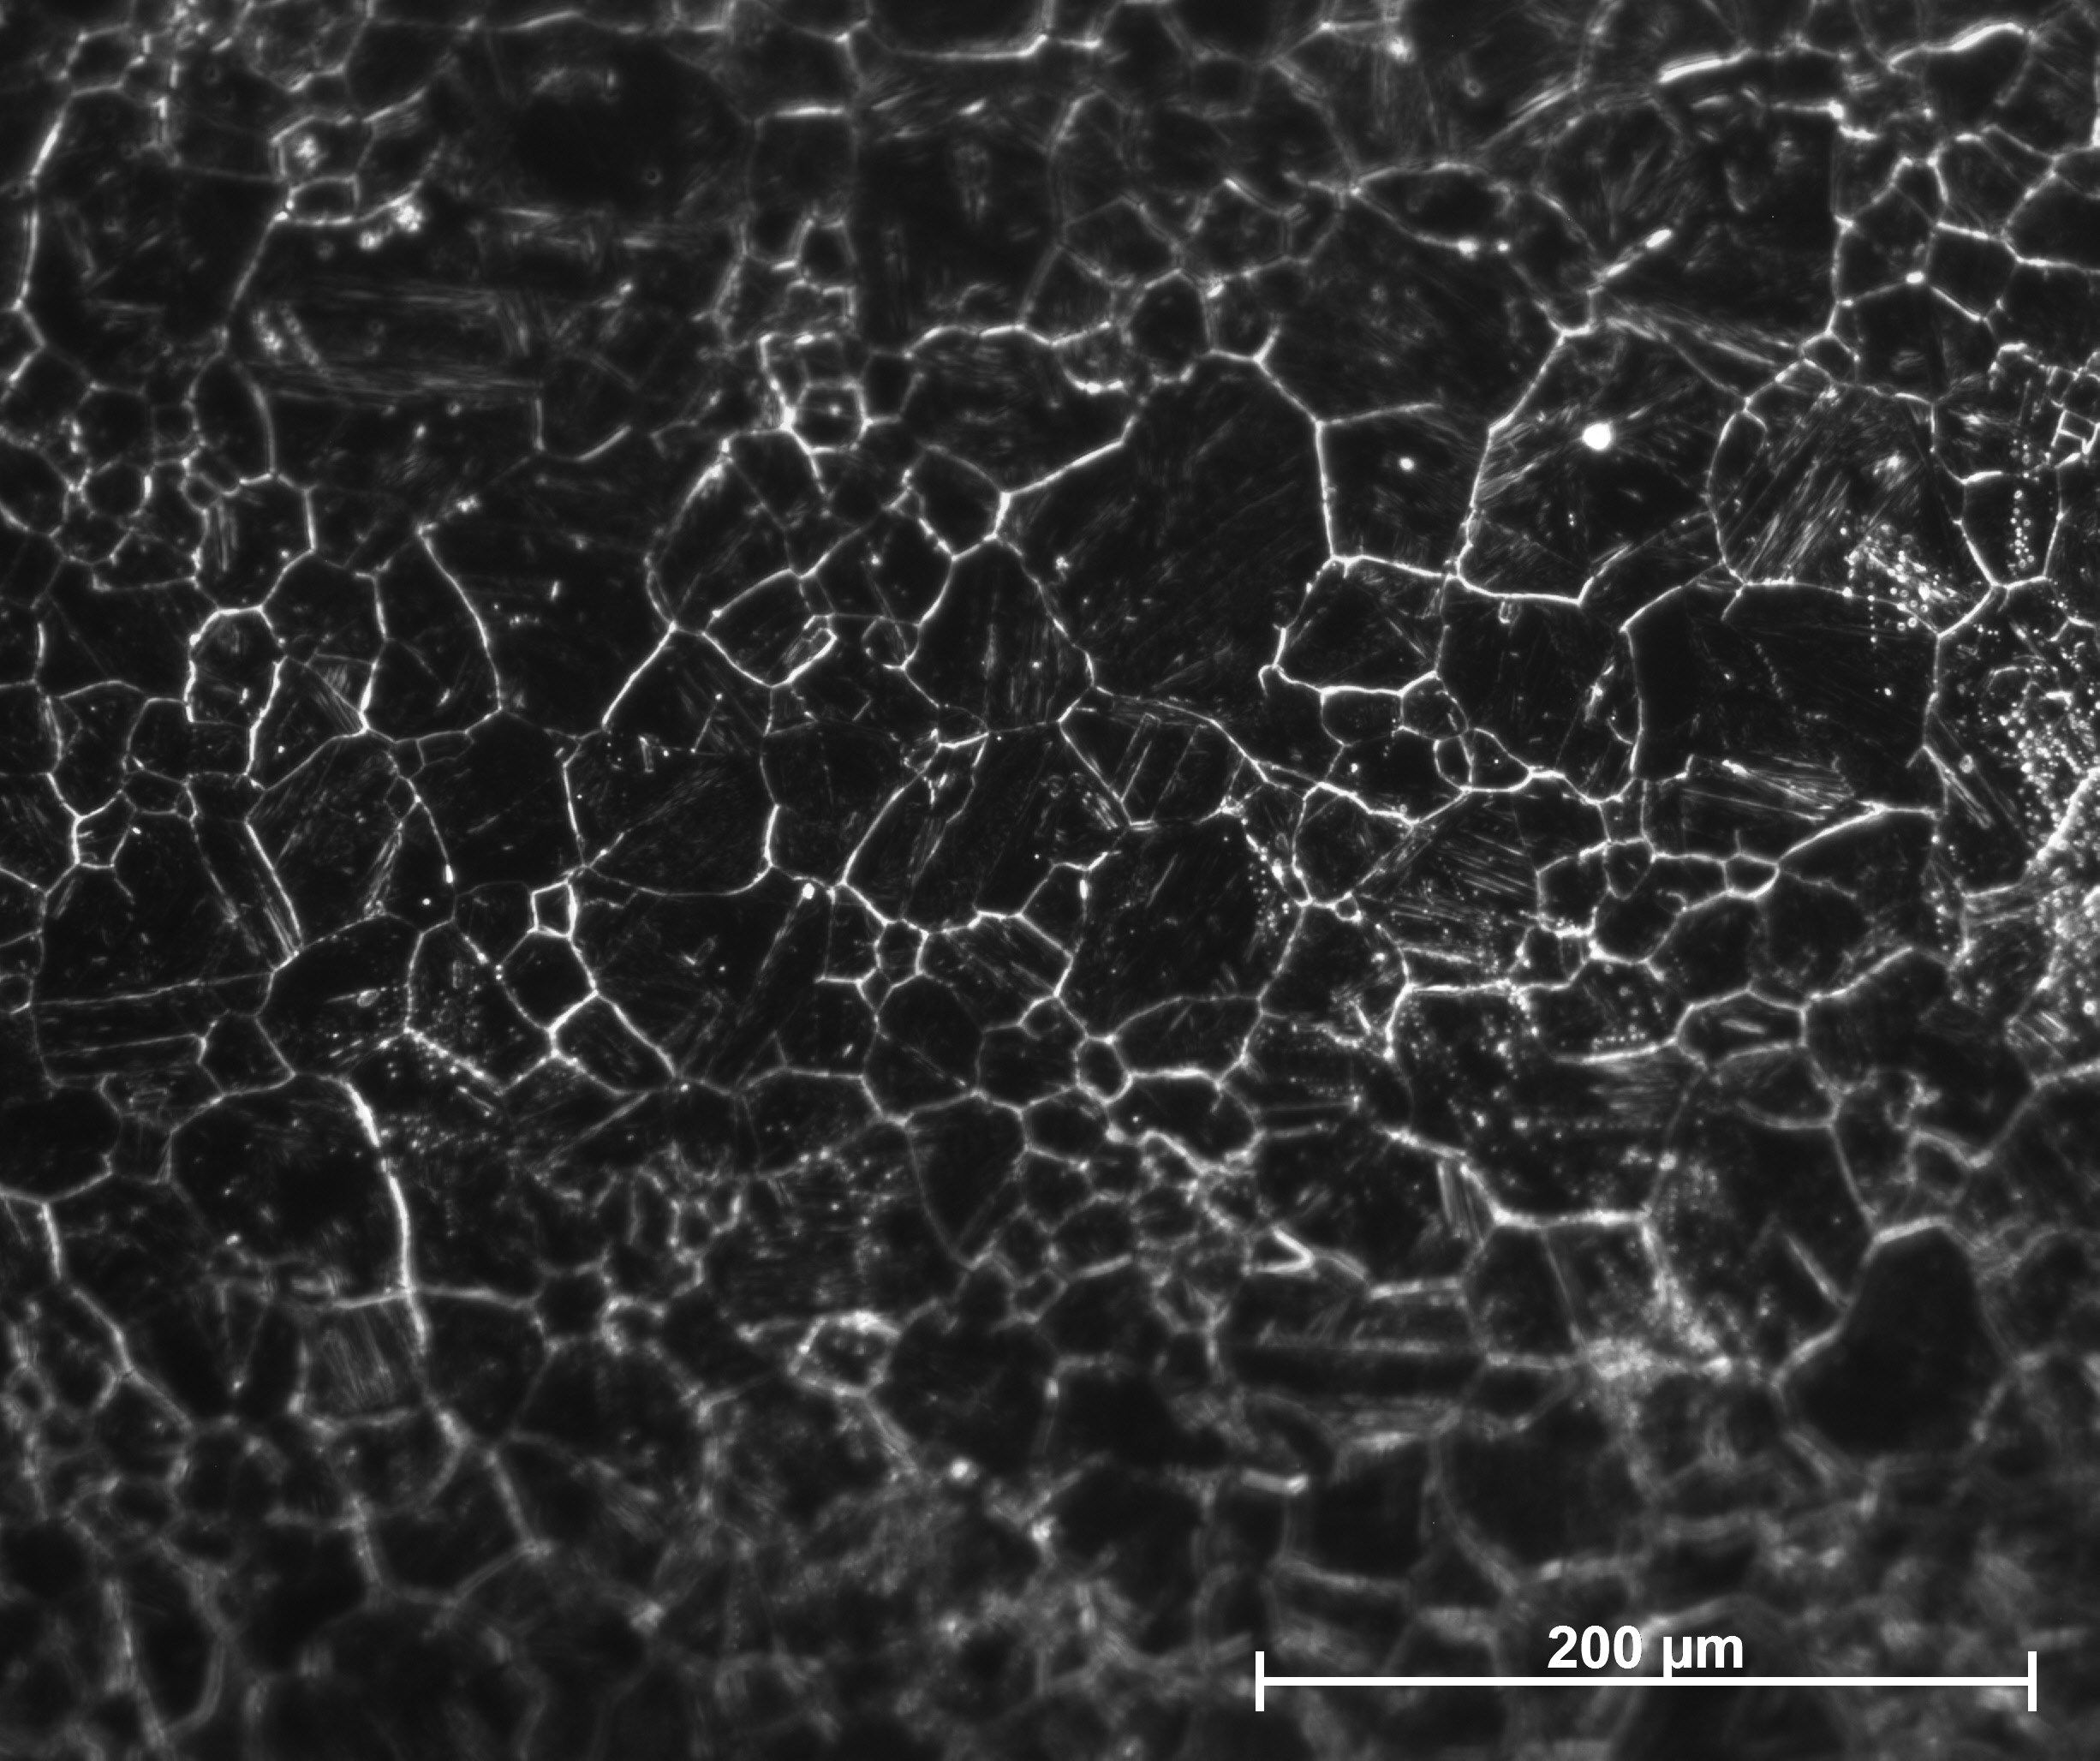
\includegraphics[width=0.9\linewidth, height=0.3\textheight]{Sa508}
    \caption{A figure showing the initial SA508 thermally etched steel microstructure image.}\label{fig:SA508}
  \end{minipage}%
  \begin{minipage}[!htb]{.5\textwidth}
    \centering\captionsetup{width=.8\linewidth}%
    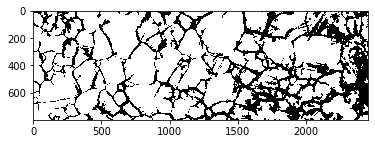
\includegraphics[width=1.0\linewidth, height=0.3\textheight]{tescase2_binary}
    \caption{A figure showing the final steel microstructure image after segmentation and processing.}\label{fig:SA508_2}
  \end{minipage}
%\caption{}\label{fig:1}
\end{figure}

\pagebreak

\noindent Test case 3 was then commenced, seeking to apply the algorithm to Figure \ref{fig:Ti64initial}, this time a brightfield image of an $\alpha$ + $\beta$ microstructure of the Ti-6Al-4V alloy, provided by Dr Pratheek Shantraj and shown below. The same procedure as in the previous test case was applied to the image and the image was successfully converted into a segmented, binary image shown in Figure \ref{fig:Ti64_2} and then exported into the Gmsh software in order to create a square based mesh for subsequent FEM analysis.\\

\begin{figure}[!htb]
  \centering
  \begin{minipage}[!htb]{.5\textwidth}
    \centering\captionsetup{width=.8\linewidth}%
    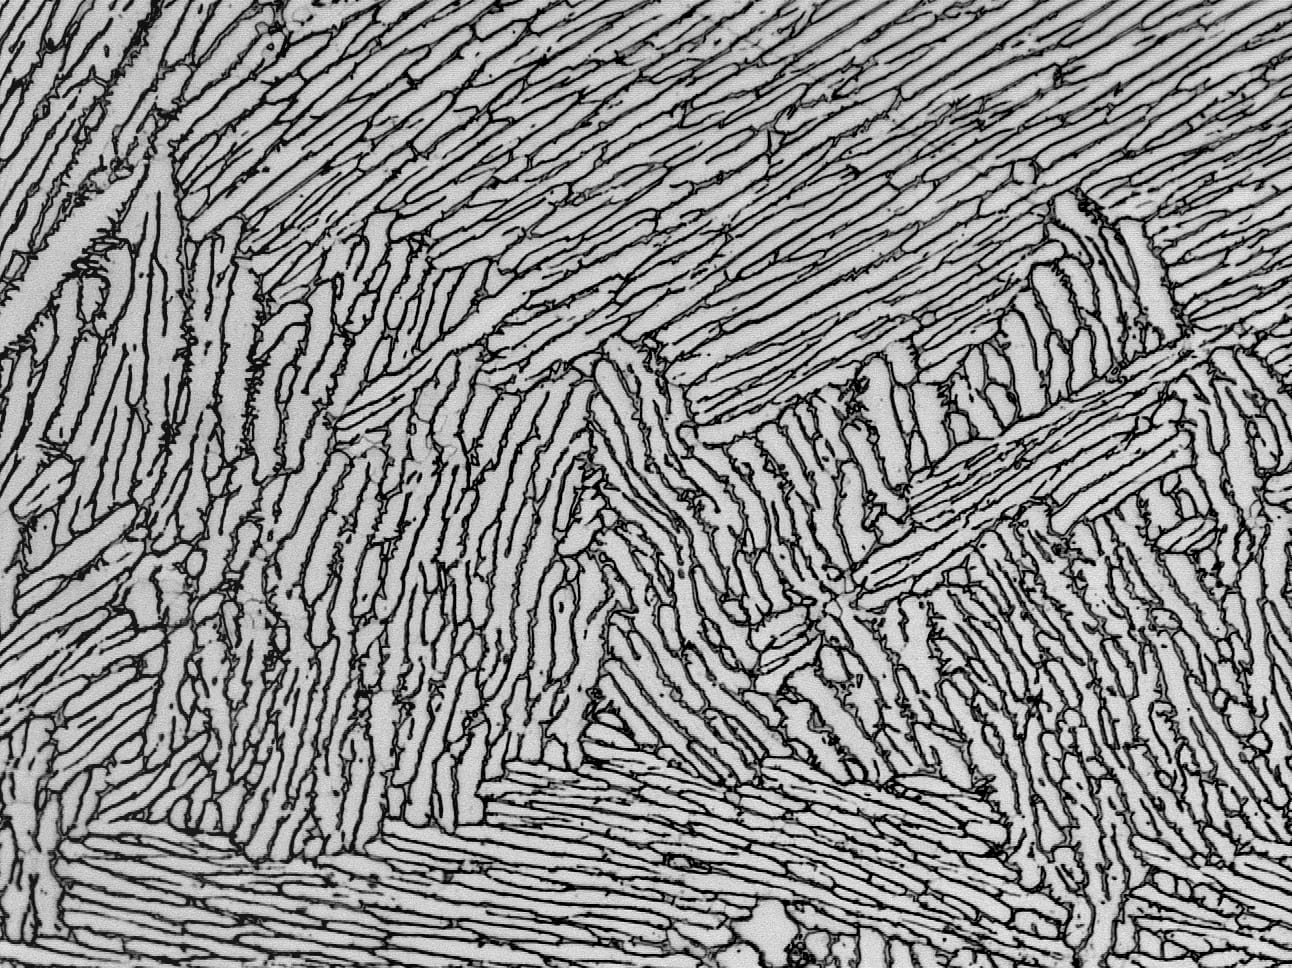
\includegraphics[width=0.8\linewidth, height=0.3\textheight]{Ti64_V1.0}
    \caption{A figure showing the initial Ti-6Al-4V microstructure image.}\label{fig:Ti64initial}
  \end{minipage}%
  \begin{minipage}[!htb]{.5\textwidth}
    \centering\captionsetup{width=.8\linewidth}%
    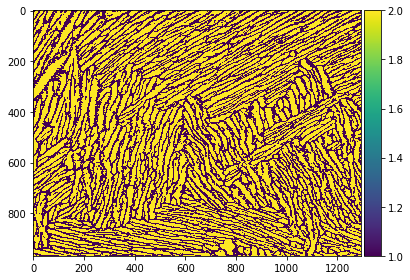
\includegraphics[width=0.9\linewidth, height=0.3\textheight]{testcase 3}
    \caption{A figure showing the final Ti-6Al-4V microstructure image after processing.}\label{fig:Ti64_2}
  \end{minipage}
%\caption{}\label{fig:1}
\end{figure}

\noindent Test case 4 then took the same image from the previous test case and processed and segmented a single grain, shown in Figure \ref{fig:Ti64single} for meshing and FEM analysis. This analysis was done with the use of the additional skimage sub-packages; threshold filters and clean border segmentation to remove the surrounding grains from the image. The binary, single grain image seen below in Figure \ref{fig:Ti64single2} demonstrates that this approach is valid for application to, and isolation of, individual grains, as well as a multitude of grains -- as demonstrated in test case 3. The successful application of the 4 test cases allowed the authors to gain a high level of confidence in the algorithm and therefore move on to the next stage of the project, meshing and FE.\\

\begin{figure}[!htb]
  \centering
  \begin{minipage}[!htb]{.5\textwidth}
    \centering\captionsetup{width=.8\linewidth}%
    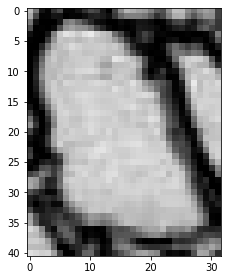
\includegraphics[width=0.7\linewidth, height=0.2\textheight]{testcase 4}
    \caption{A figure showing the initial image of a single grain of the Ti-6Al-4V microstructure.}\label{fig:Ti64single}
  \end{minipage}%
  \begin{minipage}[!htb]{.5\textwidth}
    \centering\captionsetup{width=.8\linewidth}%
    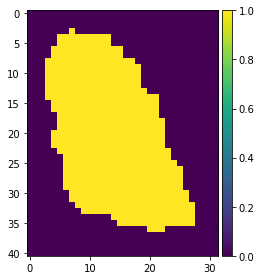
\includegraphics[width=0.7\linewidth, height=0.2\textheight]{tescase4_2}
    \caption{A figure showing the final image of a single grain of Ti-6Al-4V after segmentation and processing.}\label{fig:Ti64single2}
  \end{minipage}
%\caption{}\label{fig:1}
\end{figure}

\noindent Finally, the rigorously tested image processing code was compiled into a single function, to allow it to be easily applied to any image. The function termed 'process\_image' takes 5 input arguments and returns a binary image that can be inputted straight into the OOF2 program for meshing and simulations. OOF2 was used for the final function as opposed to Gmsh as during testing it became clear that it provided a more robust method for this particular application, which will be discussed further in the next section. The input arguments are as follows; file = the input image, e = exposure value, u/v are maximum and minimum threshold parameters respectively, and output = file name for the output file. The function therefore reads the input image, converts it to grayscale (if it is currently a rgb file) and then adjusts the exposure as per the input value of e. The Sobel filter is then applied using the values of u and v as the max/min markers to isolate grains and separate them from grain boundaries. Following this the watershed transform is applied to create a binary image which is then saved in the specified output file. The function permits the user to quickly change the input arguments and see the results easily, allowing comparisons to be made and the best possible output to be produced for the next step, meshing. Figure \ref{fig:FinalSim} shows an example of a Ti-6Al-4V microstructure image that was processed using the final function. This image would then go on to form the basis of the final simulations in the following section.

\begin{figure}[!htb]
  \centering
  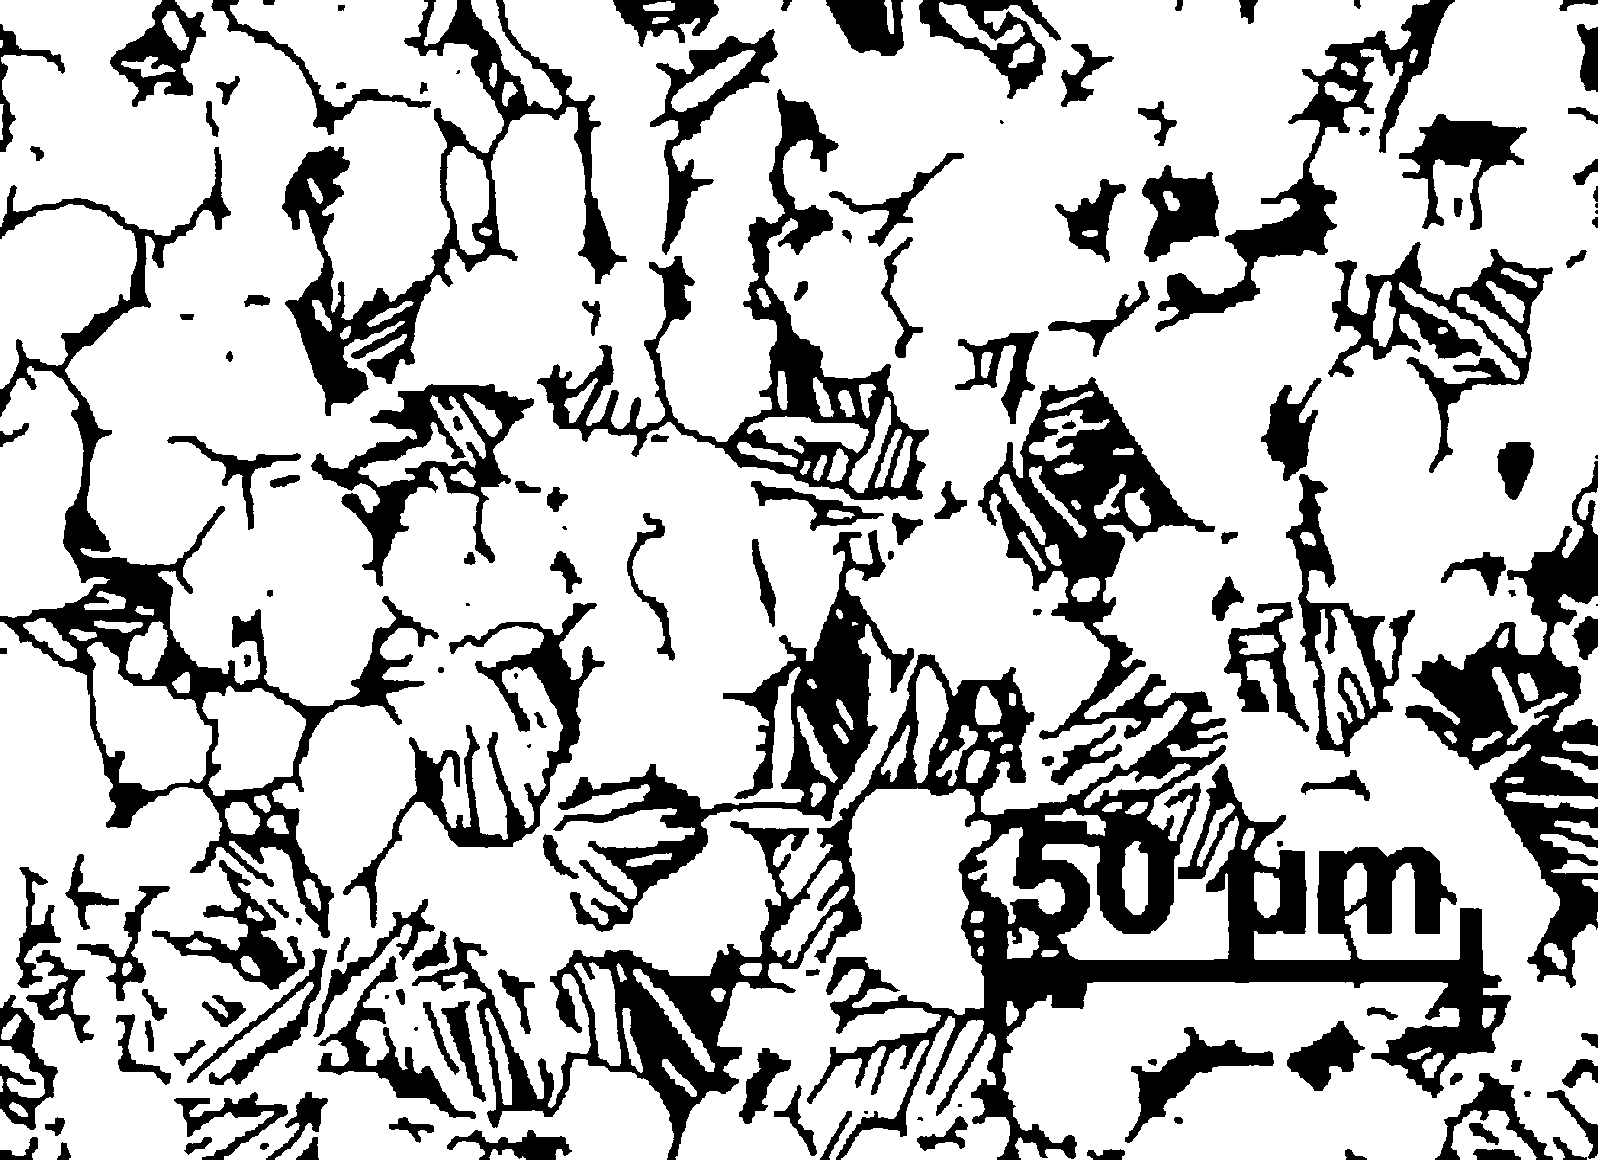
\includegraphics[width=0.8\linewidth, height=0.4\textheight]{Ti64_binary_V7.0}
  \caption{A figure showing a processed Ti-6Al-4V microstructure image that was used for the final simulation.}
  \label{fig:FinalSim}
\end{figure}

\end{document}
